The third test activity, which involved important research for the \gls{STS} is related to the testing of different relative humidity and temperature sensors. Due to the harsh conditions in the detector, the sensor's choice is an important task that will ensure the proper safety and operation of the system. This chapter presents the overview of different solutions for ambient sensing, together with answers to whether the tested technology meets all the requirements. Most efforts were made to characterize fiber optic sensors, and subsequently come up with safety requirements and systems that would address potential risks posed by e.g. too humid environment. 

\section{Sensors requirements}

The design of the \gls{STS} \cite{Heuser:54798} defines the requirements for ambient sensors. As described in the section~\ref{cooling}, the ambient temperature will reach \SI{-10}{\celsius} at the end of the \gls{STS} lifetime. The cooling liquid (3M NOVEC 649) will be circulating at temperatures close to~\SI{-40}{\celsius}. Therefore, the first boundary condition arises - the frost point needs to be below~\SI{-40}{\celsius} to avoid ice formation or condensation on the \gls{FEE}. For the first few years of operation, the temperatures will be higher and therefore RH/frost point can be measured more accurately. One of the most common techniques to achieve the frost points below~\SI{-40}{\celsius} is baking. In the case of the silicon tracker, too high temperatures could destroy the~\gls{FEE}. 
During the detector's lifetime (10 years), there will be limited opportunities to perform any upgrades. Therefore, the sensors have to withstand the radiation accumulated during that period. As some of the sensors can be placed in the vicinity of the beam pipe, the total dose could reach more than 10~kGy. The humidity measurements will be distributed, implying that different sensors may face different doses. As the detector will be placed in a dipole magnet providing a magnetic field of \SI{1}{\tesla\metre}, the sensors need to be insensitive to it. An ideal humidity sensor should meet the following requirements:
\begin{itemize}
    \item small dimensions and mass (especially when placed close to the active area of the system),
    \item accurate relative humidity readouts at temperatures down to~\SI{-20}{\celsius}, 
    \item ideally respond to a wide range of \gls{RH} values from 0~\% to 80~\%,
    \item high repeatability and low hysteresis,
    \item reliable operation across long distances (the readout device needs to reside at least~\SI{20}{\metre} away from the detector).
\end{itemize}

On the other hand, due to overpressure conditions inside the \gls{STS} enclosure, a low response time (seconds) is not necessarily needed. For the hardware and software interlocking, a delay of up to minutes is considered to be acceptable. The purpose of this chapter is to discuss the considerations for a distributed sensing system, as well as the extensive testing and design of fiber optic sensors. 
\section{Vapor pressure and its significance}

The relative humidity or the dew/frost point, are commonly used indicators to describe the number of water molecules in the air. Nevertheless, the dew/frost point is a much more useful value, as it provides an absolute value. The temperature at which water vapor in any gas medium (at constant pressure) begins to condense into liquid water or solid ice at the same rate at which it evaporates, which is a measure of how much water vapor is in a gas medium, is known as the dew/frost point. Water vapor condenses as liquid water at gas temperatures above \SI{0}{\celsius} (dew). A dew point is defined as a liquid condensation layer. Water vapor condenses as solid ice at gas temperatures far below \SI{0}{\celsius} (frost). A frost point is defined as a solid condensation layer. However, for gas temperatures ranging from \SI{0}{\celsius} to approximately \SI{-20}{\celsius}, the state of the condensed layer is unknown; it could be either water, ice, or a combination of both \cite{nie_dewpoint}. 


The first documented formula for vapor pressure (over water and over ice) was introduced by Goff and Gratch in 1945 \cite{goff_gratch}. The original correlation (over water) is as follows:

\begin{equation}
\begin{split}
    &log({e}^{*}_{s}) = a(T_{st}/T - 1) + b(log(T_{st}/T) - c(10^{11.344(1-T/T_{st})} - 1) \\
    &+ d(10^{-3.49149(T_{st}/T - 1} -1) + log(e^{*}_{st})
\end{split}
\end{equation}
where: log refers to the logarithm in base 10, $e_{s}$ is the saturation water vapor pressure~(hPa), a to d are constants; $a = - 7.90298$, $b=5.02808$, $c=1.3816*10^{-7}$, $d=1.3816*10^{-7}$, $e^{*}_{s}$ is the stream-point pressure ($1013.246~hPa$), and $T_{st}$ is the boiling point (at 1~atm) temperature (373.15~K). A similar equation can be also formulated for the vapor pressure over ice. These equations marked the beginning of the tries to formulate a highly accurate description of water dynamics. In this chapter, a highly accurate empirical formula was used to estimate the dew point. The Magnus formula is much simpler to use and allows to convert between the saturation vapor pressure and temperature with minimal error~\cite{magnus}: 
\begin{equation}
    e^{*}_{s} = c*e^{(aT/(b+T))}
\end{equation}
where: 
The \gls{RH} is usually defined as the ratio of the water vapor pressure ($p$) to the equilibrium vapor pressure over a plane of water ($p_{s}$):
\begin{equation}
    RH = 100\frac{e}{e^{*}_{s}}
    \label{eq:RH}
\end{equation}
Based of the parameters approximations by Sonntag ($c=6.112$~hPa, $a=17.62$, $b=243.12$~\SI{}{\celsius}) \cite{magnus}, the formula converges to:
\begin{equation}
    e^{*}_{s} = 6.112*e^{(17.62T/(243.12))}
    \label{eq:pressure}
\end{equation}
The dew formation corresponds to the equation:
\begin{equation}
    e^{*}_{s}(T_{d}) = e_{st}(T)
    \label{eq:dew}
\end{equation}
This approximation provides an maximum error of \SI{0.35}{\celsius} between \SI{-45}{\celsius} and \SI{60}{\celsius} in comparison to the more complex formula described in \cite{hardy}. 
Inserting the equation \ref{eq:RH} and \ref{eq:pressure} to the \ref{eq:dew} leads to the formula below, which provides the dew point in \SI{}{\celsius}.
\begin{equation}
    T_{d}(T, RH) = \frac{\lambda(ln(\frac{RH}{100})+\frac{\beta T}{\lambda + T})}{\beta - (ln(\frac{RH}{100})+\frac{\beta T}{\lambda + T}}
    \label{eq:td}
\end{equation}
The dew points based on relative humidity and temperature can be seen in the figure~\ref{fig:dewpointmagnus}.
\begin{figure}[!h]
\centering
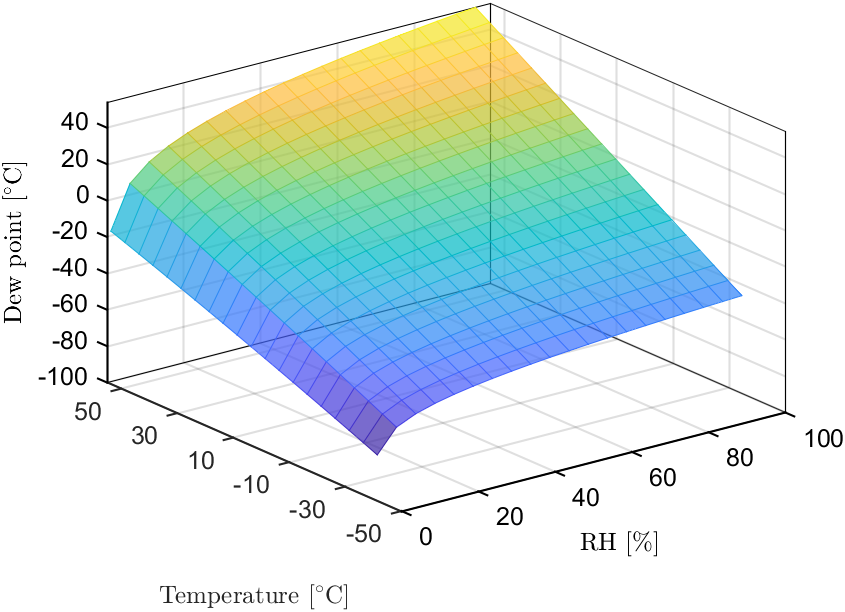
\includegraphics[width=0.65\columnwidth]{Chapter5/images/dewpointmagnus.png}
\caption{Dew points calculations based on the empirical formulas}
\label{fig:dewpointmagnus}
\end{figure}
In order to compare the results of different relative humidity sensors and dew points sensors, uncertainties of the \footnote{"Dry Bulb Temperature" refers essentially to the ambient air temperature. It is called "Dry Bulb" because the air temperature is indicated by a thermometer not affected by the moisture of the air.}{dry-bulb} temperature and \gls{RH} are needed. In uncertainty analysis, the individual standard uncertainty $\mu$ is defined as the uncertainty of the result of a measurement expressed as its standard deviation~\cite{NIST_1994}. Hence, assuming the rectangular uncertainty for the sensors that measure the temperature and relative humidity:
\begin{equation}
    \mu(x_{i}) = \frac{a}{\sqrt{3}}
\end{equation}
where a is the uncertainty available in the datasheets, and $u_{i}$ represents the measured value. The combined uncertainty $\mu_{c}$ can be derived from equation \ref{eq:dew} based on the law of propagation of uncertainty~\cite{dp_uncertainty}:
\begin{equation}
    u_{Td} = \left [  \left (\frac{\partial T_{d}}{\partial T_{a}}  \right )^{2} \mu^{2}(T) + \left (\frac{\partial T_{d}}{\partial RH}  \right )^{2} \mu^{2}(RH)\right ]^{1/2}
    \label{dp_error}
\end{equation}
In each system, we assume that measuring dew point temperature or relative humidity is statistically independent of measuring air temperature and the confidence level for the uncertainty interval is 68~\%.  Moreover, below~\SI{0}{\celsius} the frost point starts to play a key role. The moisture in the air will undergo deposition as a layer of frost on exposed surfaces that are also at a temperature below the frost point. 

\section{Overview of different technologies}

Nowadays electronic humidity sensors are commonly used in industry, scientific research facilities, and civil infrastructure. In general, we can divide the sensors based on their operating principle - changes in current, voltage, weight, or conductivity can be subsequently associated with humidity changes if the underlying detection principles relate to interaction with water. Resistive and capacitive sensors represent over 75~\% of all sensors used today. As the names indicate their working principles are based on capacitance and resistance changes respectively. The two most difficult requirements to be met are radiation hardness and insensitivity to the magnetic field. Radiation can affect sensor materials in different ways depending on their type, rate of interaction, and material composition. Sensor structures are affected by radiation due to modifications to their lattice structures. For example, capacitive sensors like HIH3610 and HIH4030 tested in CERN turned out to be critically damaged after irradiation~\cite{Berruti} On the other hand, recently it was also reported that capacitive sensors from IST AG has a linear response to the radiation, what can be easily corrected~\cite{Kapic_sensor}. Employing such sensors in a \gls{HEP} experiment, especially in a tracker which is surrounded with a magnet raises questions about the sensitivity to the magnetic field. One of the possible solutions is using fiber optic-based sensors which are by design not sensitive to the changing magnetic field. Another possibility would be to transfer the air from the detector enclosure to measure it outside of the magnetic field, in an area without elevated dose. 

The efforts to employ miniaturized sensors in the \gls{HEP} experiment have been ongoing for many years \cite{Berruti}. A general review of the dew point and relative humidity sensing techniques was presented in~\cite{RITTERSMA}. On the other hand, a more recent overview with a case-specific study related to \gls{HEP} is summarized in \cite{Kapic}. The \gls{STS} will feature a few different technologies of the \gls{RH} and temperature sensors - capacitive sensors, fiber optic sensors and dew point transmitters. 


\subsection{Industrial capacitive sensors}
The capacitive sensors, in the simplest form, can be made out of two parallel plates, where the capacitance between the two electrodes in given by:
\begin{equation}
C = \epsilon_{r}\epsilon_0\frac{A}{d}
\end{equation}
where the $\epsilon_{r}$ and $\epsilon_{0}$ are the relative and vacuum permittivity constant, A is the plate surface area and d is the plate distance. If the humidity changes can be associated to the changes of one of the parameters a \gls{RH} can be therefore calculated. 
The capacitive \gls{RH} sensors can measure below \SI{0}{\celsius}, they are fairly miniaturized and insensitive to pressure changes. The main drawbacks of these sensors are listed below:
\begin{itemize}
    \item limited long-term stability,
    \item sensitive to water condensation,
    \item limited distance to the readout device,
    \item most of the sensors are not radiation-hard.
\end{itemize}
Two different \gls{RH} capacitive sensors have been tested in low-temperature regimes - IST HYT221 and Sensiron SHT85. Figure \ref{fig:hyt221} shows the \gls{RH} and temperature error respectively. Measuring humidity at low temperatures below \SI{-20}{\celsius} and 5~\% \gls{RH} leads to large dew point errors (\SI{7}{\celsius} and more). The estimated dew point errors are presented in figure \ref{fig:hyt221_dp}.
\begin{figure}[!h]
\centering
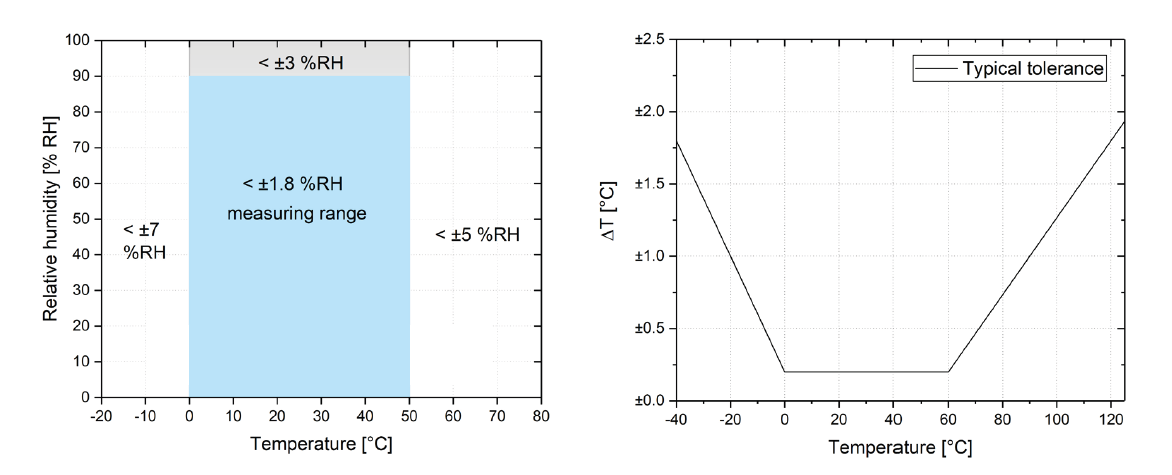
\includegraphics[width=0.85\columnwidth]{Chapter5/images/hyt221_rh.png}
\caption{Relative humidity and temperature uncertainties \cite{hyt221}}
\label{fig:hyt221}
\end{figure}
\begin{figure}[!h]
\centering
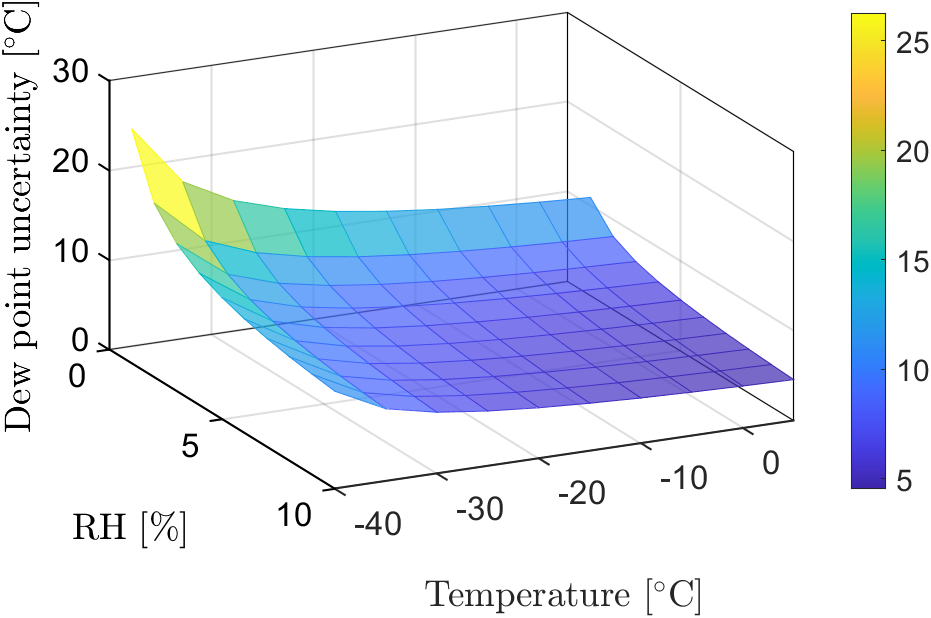
\includegraphics[width=0.6\columnwidth]{Chapter5/images/HYT221RH7T15.png}
\caption{Dew point error based on values from the figure \ref{fig:hyt221}}
\label{fig:hyt221_dp}
\end{figure}
\newpage
Figure \ref{fig:sht85} shows the uncertainties for the measurements with the SHT85 sensor above \SI{0}{\celsius}. The data below \SI{0}{\celsius} is not provided, therefore an extrapolation was made in order to have a comparison with the HYT221 sensor. The results are presented in the figure~\ref{fig:sht85_dp}. In this case, the errors reach up to \SI{7}{\celsius} in the lowest temperatures and \gls{RH} levels.
\begin{figure}[!h]
\centering
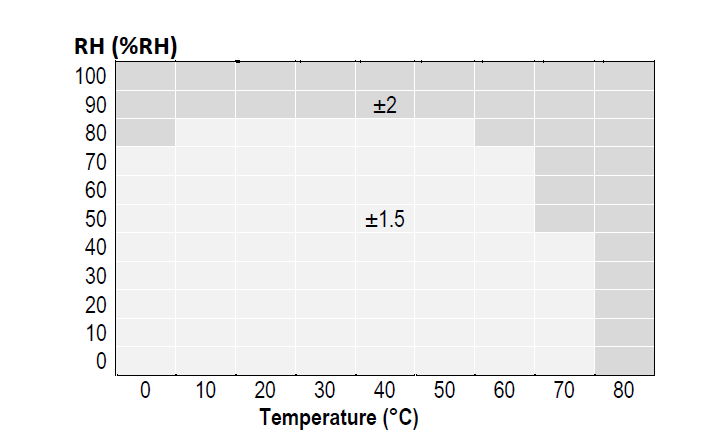
\includegraphics[width=0.65\columnwidth]{Chapter5/images/sht85_rh.png}
\caption{Relative humidity uncertainties, the temperature uncertainty is \SI{0.2}{\celsius} \cite{SHT85}}
\label{fig:sht85}
\end{figure}

\begin{figure}[!h]
\centering
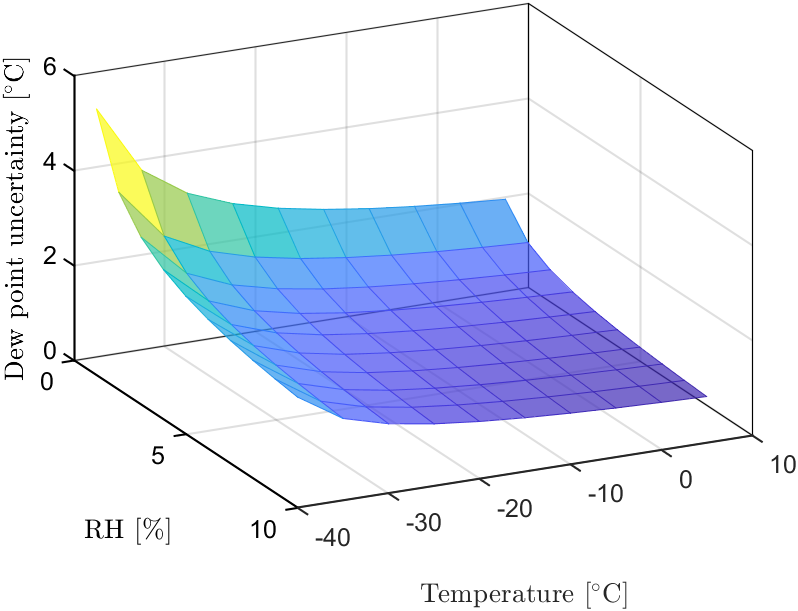
\includegraphics[width=0.6\columnwidth]{Chapter5/images/SHTRH15T02.png}
\caption{Dew point error based on the the figure \ref{fig:sht85}}
\label{fig:sht85_dp}
\end{figure}
\newpage
The results presented above don't take into consideration additional effects that alter the dew point results, like hysteresis or drift, which could together contribute by 1~\% or more to the \gls{RH} measurement. Moreover, the performance of the SHT85 is most likely also worse in the low-temperature regime. The comparison of the industrial capacitive sensors shows a large performance disproportion which is also reflected in the price. In general, the industrial capacitive sensors are much cheaper than the custom trace humidity measurement systems or fiber optic sensors. Nevertheless, the readout of such sensors may be affected by the radiation and magnetic field, so they can't be considered as a reliable solution for a long-term operation in the \gls{STS}. The next type of sensors that yield promising results is fiber optic sensors~\ref{FOS}.

\subsection{Fiber optic sensors}
\label{FOS}
Optical fiber optic sensors-based system usually consists of three main components as optical source, transducer, and detector. In general, the sensing principle relies on modifying one or more properties of light (most commonly a laser, diodes, or LEDs are employed as the optical sources) passing through a transducer which is located inside the fiber. A schematic view of a sensing setup is presented in the figure~\ref{fig:sensing}.  The mentioned figure highlights also another feature of this technology, distributed sensing or even continuous sensing offers the unique opportunity for many sensing points in one fiber~\cite{GRATTAN200040}. 
\newpage
\begin{figure}[!h]
\centering
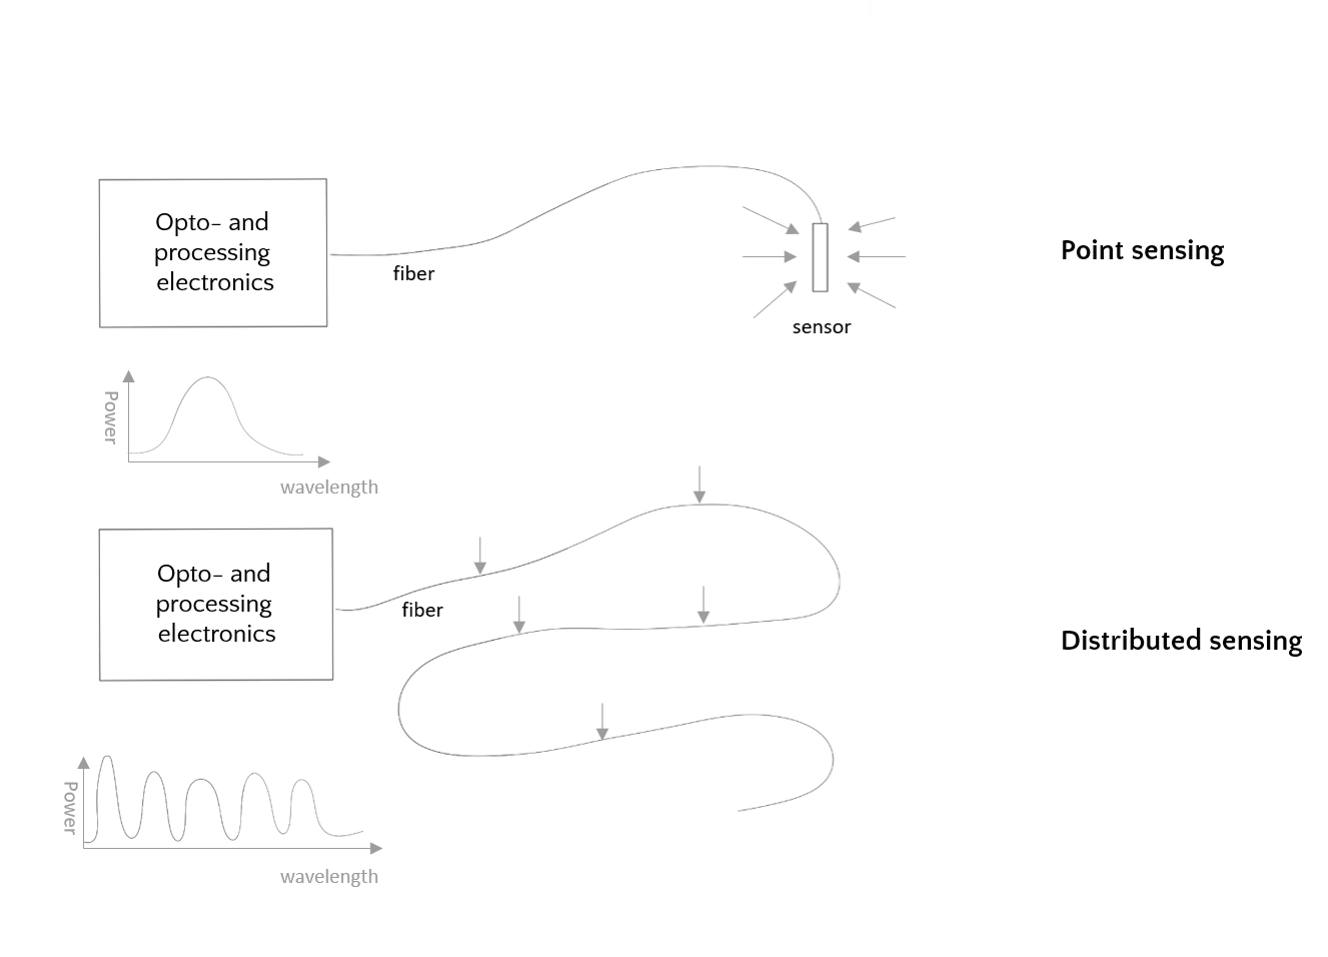
\includegraphics[width=0.95\columnwidth]{Chapter5/images/sensing.png}
\caption{Comparison of different sensing possibilities with the \gls{FOS}}
\label{fig:sensing}
\end{figure}

In general, humidity sensing can be classified according to the operating principles being used \cite{fos_overview}. Furthermore, we can distinguish intrinsic and extrinsic sensors that indicate whether sensing occurs inside or outside of the fiber. The main effort has focused on in fiber grating sensors, which belong to a class of intrinsic \gls{FOS} that has gained popularity in recent years. As a result, we initially focused on a technology called Fiber Bragg Grating. The driving factor for this decision was the successful implementation of the sensors in the Compact Muon Solenoid (\gls{CMS}), which was extensively reported in a number of papers and summarized in the PhD thesis~\cite{Berruti}.

Fiber optic sensors have notable advantages in comparison to conventional sensors:

\begin{itemize}
    \item fibers can be insensitive to radiation or have a predictable behavior,
    \item magnetic field insensitive,
    \item good signal transmission over long distances,
    \item multiplexing capabilities (see figure~\ref{fig:sensing}),
    \item immunity to electrostatic and electromagnetic interference,
    \item resistant to harsh conditions - the sensors are completely passive elements, hence they offer long durability.
\end{itemize}
On the other hand, \gls{FOS} are difficult to integrate into hardware interlocks, and handling and installation of the sensors might be more challenging due to the risk of damaging the fiber.




\subsubsection{Fibre Bragg Grating based sensors}

Fiber Bragg Grating is a type of selective filter that reflects light signals at a specific wavelength known as the Bragg wavelength. Such a filter is created by inscribing a systematic variation of the refractive index~\cite{fbg_overview}. This characteristic wavelength ($\lambda_{B}$) is dependant on the fiber effective refractive index ($\eta_{eff}$) and the grating pitch ($\Lambda$) of the \gls{FBG}~\cite{Othonos2000FiberBG}:
\begin{equation}
    \lambda_{B} = 2 \eta_{eff} \Lambda
\end{equation}
Both factors can be affected by strain, temperature, magnetic field, and/or pressure changes, which makes them a viable choice for sensing applications~\cite{Yun-Jiang_Rao_1997}. In general wavelength shift $\lambda_{B}$ can be formulated as:
\begin{equation}
    \frac{\Delta\lambda_{B}}{\lambda_{B}}=(1-P_{e}) \epsilon + \left [(1-P_{e}) \alpha + \xi  \right ] \Delta T
\end{equation}
where $P_{e}$ is a photo-elastic constant, $\epsilon$ is a strain induced on the fiber, $\alpha$ is the thermal expansion coefficient of the coated \gls{FBG}, and the $\xi$ is the thermo-optic coefficient of the fiber. Using an \gls{FBG} temperature sensor requires decoupling the strain measurement from the temperature measurement, usually called temperature compensation~\cite{Yun-Jiang_Rao_1997}. The most commonly used solution involves using two sensors next to each other or inscribed in the same fiber. The first sensor is responsible for measuring the strain, and the second one measures the temperature in strain-free conditions. The wavelength shift $\Delta \lambda$ induced by the $\Delta T$ can be described as:
\begin{equation}
    \frac{\Delta\lambda_{B}}{\lambda_{B}}=\left [(1-P_{e}) \alpha + \xi  \right ] \Delta T
\end{equation}


\begin{figure}[!h]
\centering
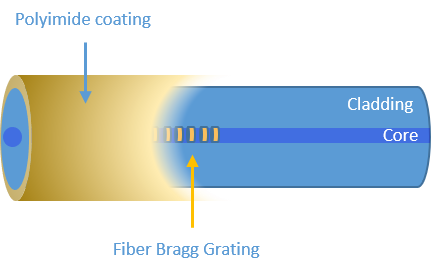
\includegraphics[width=0.45\columnwidth]{Chapter5/images/Picture1.png}
\caption{FBG-based sensors for relative humidity measurements}
\label{fig:fbg_scheme}
\end{figure}


It's possible to measure RH instead of strain by applying a hygroscopic material (for example, polyimide) to the fiber cladding (see figure~\ref{fig:fbg_scheme}. The  Bragg wavelength shift becomes a superposition of temperature and humidity effects in this case (see equation (see equation~\ref{eqn:FBG})~\cite{Kronenberg:02, YEO2008280}. 
                            %\newpage
                             \begin{equation}\label{eqn:FBG}
                            %\large
                                    \frac{\Delta\lambda_{B}}{\lambda_{B}}=\Delta TS_{T}+\Delta RHS_{RH}
                            \end{equation}
                            where $\lambda_{B}$ is the Bragg wavelength, and $S_{RH/T}$ are the sensitivity coefficients for RH and temperature, respectively. 

Similarly to the strain measurement, it’s crucial to have precise temperature readouts in the vicinity of the coated \gls{FBG}. Otherwise, the actual RH readout may be dominated by uncertainty or just the inaccurate temperature measurement. \gls{FBG} sensors should also be packaged appropriately and kept strain-free to prevent additional stress. Detailed discussion about the experimental setup, chosen design of the \gls{FBG} sensors, and their features will be presented in the section~\ref{fbg_results}.



\subsection{Trace humidity sensing}
Due to expected very low dew point levels inside the \gls{STS} (below \SI{-45}{\celsius} and the requirement to keep the device safe, it was proposed to use trace humidity sensors in so-called sniffing system~\cite{Berruti}.
The most common sensing techniques include:
\begin{itemize}
    \item tunable diode laser (dew points up to \SI{20}{\celsius}),
    \item oscillating quartz crystal sensor (dew points up to \SI{0}{\celsius}),
    \item aluminum oxide sensor (dew points up to \SI{20}{\celsius}),
    \item chilled mirror dew point hygrometer  (dew points up to \SI{100}{\celsius}).
\end{itemize}
As such most of them include digital circuitry in the active area, which could be affected both by radiation and magnetic field, therefore a special system with a vacuum pump was chosen~\ref{fig:sniffer}. 

\begin{figure}[!h]
\centering
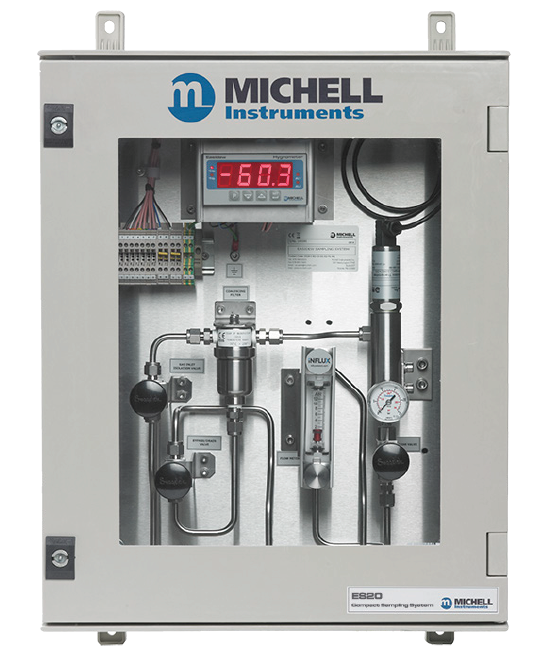
\includegraphics[width=0.35\columnwidth]{Chapter5/images/ES20.png}
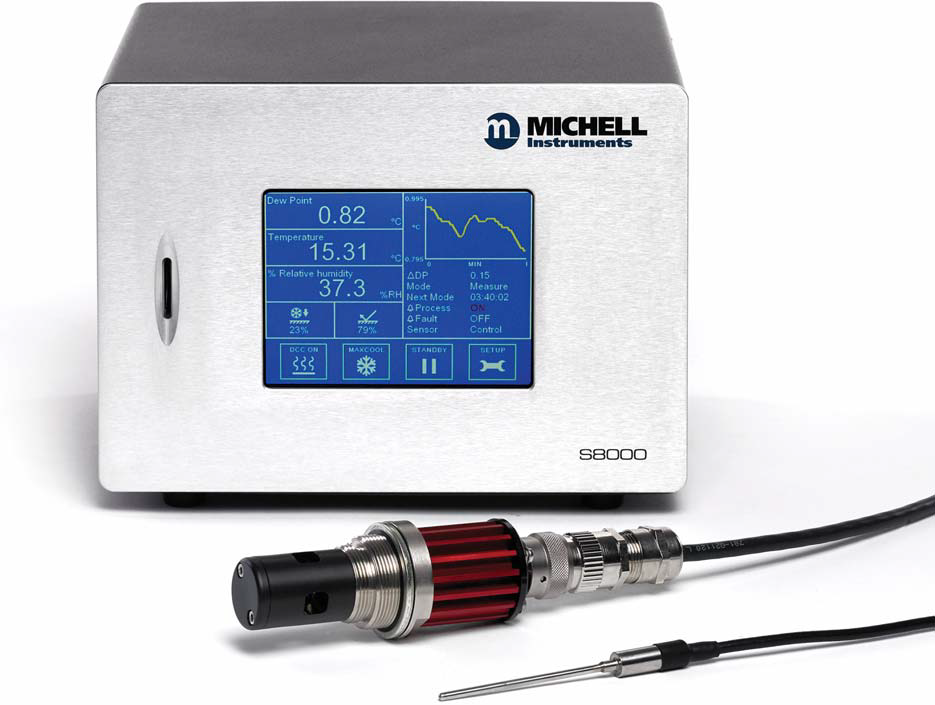
\includegraphics[width=0.4\columnwidth]{Chapter5/images/s8000.png}
\caption{Left: Michell ES20 ceramic metal-oxide sampling system~\cite{michell_e20}
Right: Michell S8000 Remote High Precision Chilled Mirror Hygrometer~\cite{michell_s8000}}
\label{fig:sniffer}
\end{figure}
Aluminum oxide interacts with water, and it is considered a sensitive layer and is used for moisture sensors. The best way to compare the sensor is to do that with a capacitor. The sensors are characterized by very low uncertainties, and the implementation in a hardware-based interlock is much easier than in the case of the \gls{FOS}.

Another precise and commonly used method is the chilled mirror hygrometer. In this method, a mirror is cooled slowly and in a controlled manner until condensate can be detected on it. Using a vapor pressure curve, we can determine the partial pressure of water vapor at the dew point of flowing gas. A careful measurement presupposes that equilibrium conditions are reached. This can only be achieved by approaching the dew point approximately with the temperature regime and repeating it several times. The measurement range of the Michell S8000 chilled mirror is presented in the figure~\ref{fig:fos_mirror}. The hygrometer together with the HYT221 and SHT85 was used to calibrate and characterize FBG-based \gls{FOS}. 

\begin{figure}[!h]
\centering
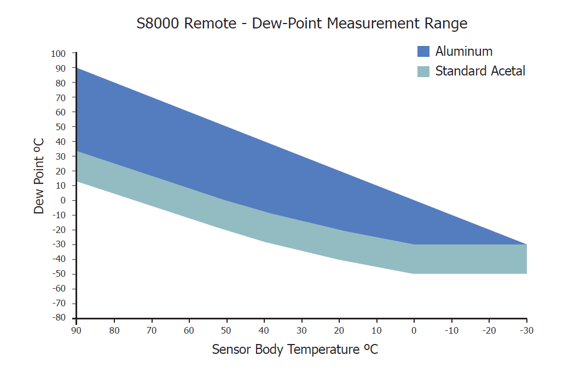
\includegraphics[width=0.65\columnwidth]{Chapter5/images/s8000_remote.png}
\caption{Controls architecture for the temperature and humidity sensor measurement}
\label{fig:fos_mirror}
\end{figure}
\newpage
\subsection{Performance in high radiation environments}
Implementing a cost-effective distributed sensing system is a challenging task. Sniffing lines that suck air samples from the detector's active area, and then the trace humidity sensors measure the dew point in a distant (safe) area, are considered to be the most reliable way, but their cost per sensing point is relatively high. 

Over the years, the capacitive sensors have been widely used in many industrial applications, but their susceptibility to radiation, doesn't qualify them as appropriate and reliable sensors for long-term \gls{STS} operation~\cite{Kapic, capacitive_irrad, Berruti}.  RH sensors based on polymer are mainly affected by ionizing radiation. The sensor's internal electronic circuit is its most vulnerable part~\cite{SHCHEMEROV20222871}.

In recent decades, researchers have studied the effects of different types of radiation on optical fibers. When radiation interacts with materials, it changes their characteristics and often affects the performance and reliability of the devices, with pronounced consequences. For all these reasons careful investigations concerning how the radiation affects the operation of components intended for use in these harsh environments were conducted. The radiation may cause point defects inside the fiber, causing the attenuation of the signal~\cite{FOS_FIB_RAD}. Nowadays, it's possible to to fabricate radiation hard fibers \cite{troska}, for example as reported in \cite{Berruti} commonly used Corning SMF-28 optical fibers are considered radiation tolerant. However, a careful choice of the fiber material is needed, as it reliability depends on many factors as dose, dose rate, wavelength.  Another matter that needs to be considered is the influence of the radiation on the Fiber Bragg Grating, as the radiation may affect the wavelength shift~\cite{gusarov}. The grating itself survives high doses, but it's no completely insensitive to the particles flux. Similarly as with the fibers, many factors can influence the response to the radiation of the grating. Some of them like the doping concentration in the fiber and hydrogen laoading 



\section{Experimental setup}
The experimental setup consists of several devices, listed in the figure~\ref{fig:fos_arch}. 

\begin{figure}[!h]
\centering
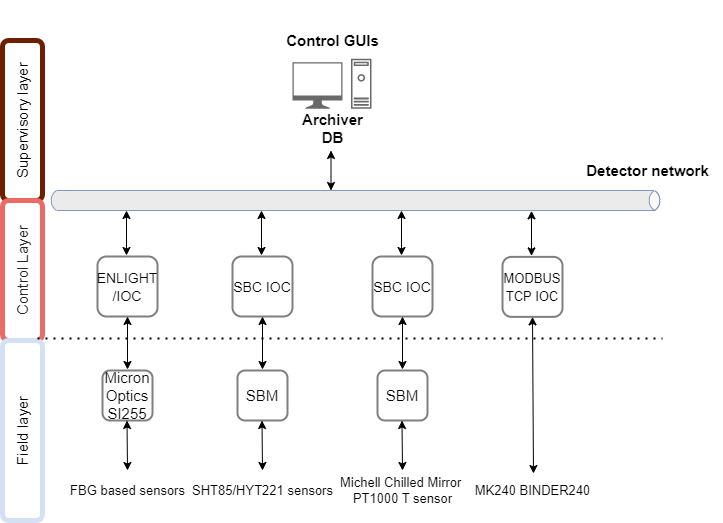
\includegraphics[width=0.75\columnwidth]{Chapter5/images/FOS_dcs_scheme.png}
\caption{Controls architecture for the temperature and humidity sensor measurement}
\label{fig:fos_arch}
\end{figure}

